

%%%%%%%%%%%%%%%%%%%%%%%%%%%%%%%%%%%%%%%%%%%%%%%    
\subsection{Exercise 2 - Madeline Brandt}
 
In this chapter, we study the tropicaliztion of genus 2 curves. Given a genus 2 curve $C$ over a valued field $K$, there is a genus 2 tropical curve we can associate to $C$ uniquely. This is the dual metric graph of the special fiber of a semistable model for $C$, with appropriate edge lengths. This is also the Berkovich skeleton of the Berkovich analytification of $C$.
It is a nontrivial task compute this tropical curve, and the problem has been studied in the papers \cite{masters} and \cite{section5}, each using a different method. In what follows, we will discuss both methods and provide examples which demonstrate that the two methods yield the same results.


\subsubsection{Moduli Space of Tropical Curves}

For our purposes, a \emph{tropical curve} will be a triple $(\Gamma, w, l)$ where $\Gamma = (V,E)$ is a connected graph, and $w$ is a function from $V\rightarrow \mathbb{Z}_{\geq 0}$ assigning weights to the vertices, and $l$ is a function from $E \rightarrow \mathbb{R}_{\geq 0}$ assigning a length to each edge. The genus of a tropical curve is the sum over all weights of the vertices, plus the classical genus of the graph $\Gamma$. We will say that two tropical curves are isomorphic if one can be obtained from the other via the following operations:
\begin{enumerate}
\item Graph automorphisms.
\item Removing a leaf of weight 0, together with the edge connected to it.
\item Removing a vertex of degree 2 and weight 0, and replacing the corresponding edges by one edge whose length is the sum of the lengths of the old edges.
\item Removing an edge of length 0 and adding the weights of the corresponding vertices.
\end{enumerate}
In this way, every tropical curve has a \emph{minimal skeleton}. This is a tropical curve with no vertices of weight 0 and degree less than or equal to two, or edges of length zero.

Given a fixed pair $(\Gamma, w)$, or \emph{combinatorial type}, the moduli space of tropical curves of this type is given by $\mathbb{R}_{\geq 0}^{|E|} / \text{Aut}(\Gamma)$. The coordinates in $\mathbb{R}_{\geq 0}^{|E|}$ give the edge lengths in the graph. The boundary of these cones corresponds to curves with at least one edge of length 0. Then, we glue the cones along the boundaries to form $M_g^{tr}$. The moduli space  $M_g^{tr}$ is a \emph{stacky fan}, and has been well studied. This is a fan together with some identifications, as described above. The stacky fan $M_2^{tr}$ is displayed below.

 \begin{figure}[h]
\centering
  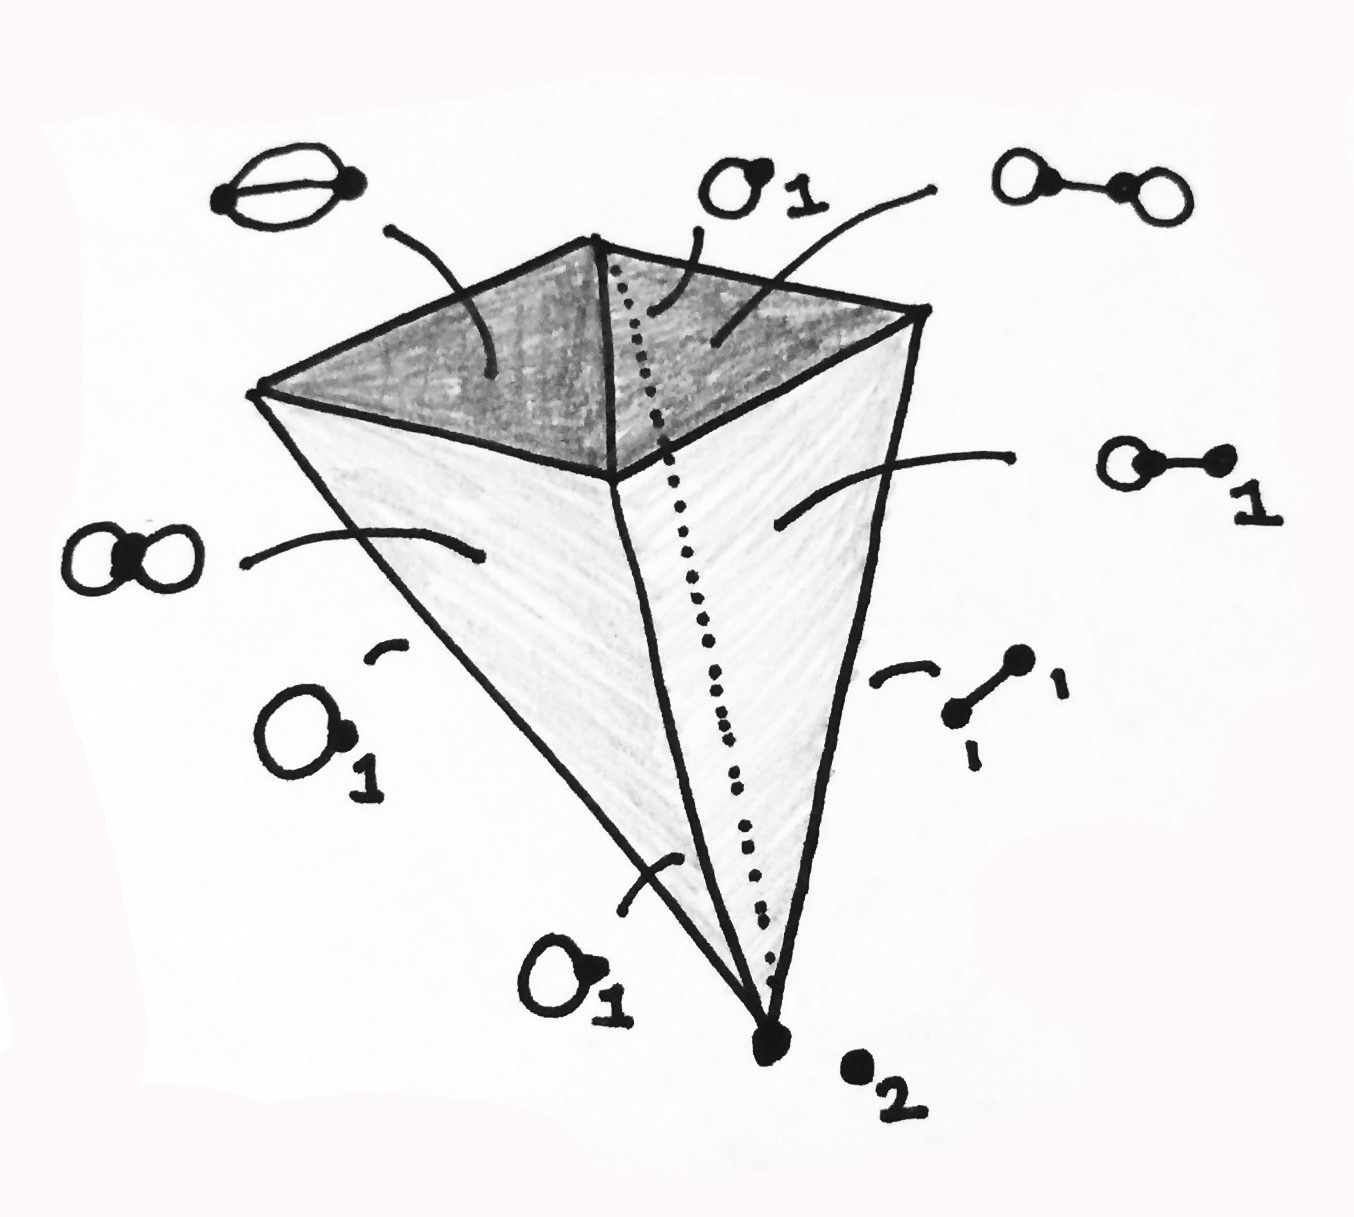
\includegraphics[width=.5\linewidth]{mgtrop2}
  \caption{The moduli space $M_2^{tr}$ of genus 2 tropical curves.}
  \label{mgtrop}
\end{figure}

\subsubsection{The dual graph of a curve}
We have that there exist coarse moduli spaces $\overline{M}_g$ and $\overline{M}_{g,n}$ of stable curves and $n$-pointed stable curves, and each is a projective variety. These are called the \emph{stable compactifications} of $M_g$ and $M_{g,n}$. The space $\overline{M}_g$ is compact and separated.
The evaluative criterion for properness tells us that any regular map from the complement of a point on a smooth curve to $\overline{\mathcal{M}}_g$ admits an extension to a regular map on the whole curve. The separability can be thought of as showing that this extension is unique. 

In what follows we will describe how to map curves over a valued field to tropical curves. Let $R$ be a complete discrete valuation ring with maximal ideal $m$. Let $K$ be the field of fractions of $R$, and let $k = R/m$ be the residue field. Let $t \in R$ be a uniformizing parameter. Fix a genus $g$ curve $C$ over $K$. The curve $C$ gives a morphism from $\text{spec}(K) \rightarrow M_{g}$. Since $\overline{M}_g$ is proper, a stable curve over $K$ uniquely extends to a stable curve $C / \text{spec}(R')$, where $R'$ is the valuation ring of a finite extension $K'$ over $K$. Then, we have a morphism $\text{spec}(R') \rightarrow \overline{M_{g}}$. This is called a \emph{stable model} of $C$. Reducing modulo $m'$ gives a map $\text{spec}(k) \rightarrow \overline{M_{g}}$. Then this is a stable curve $C_S$ over $k$. The stable model may not be unique, but the stable curve is unique. This curve has at worst nodal singularities.

We will define the dual tropical curve as follows. Given a stable model for $C$, the vertex set of the graph will be the collection of irreducible components, where each vertex has a weight equal to the genus of the components it came from. For each node, make an edge between the corresponding vertices. Given a vertex-weighted graph $\Gamma$, the genus of $\Gamma$ is the sum over all weights of the vertices, plus the classical genus of the graph $\Gamma$. Then, if $\Gamma$ is the dual graph of a curve $C$, it has the same genus as $C$. We will discuss how to obtain the length function (to make this a metric graph).
Given an edge $e$ in $\Gamma(C_S)$, we have a node $p \in C_S$. Near $p$, the curve $C_S$ admits a local equation of the form $xy=f$, for $f \in R$. Let $l(e) = val(f)/d$, where $d$ is the degree of the field extension $K \subset K'$. We note that this is independent of the local equation chosen. Now, we have a tropical curve $(\Gamma(C_S), l)$. \\

 Let $M_{\Gamma}$ be the space parametrizing curves with weighted graph $\Gamma$. Then its codimension in $\overline{M}_g$ is equal to the number of edges in $\Gamma$, and we have that
$$
\overline{M}_g = \bigsqcup_{\Gamma\text{ st }g(\Gamma)=g} M_\Gamma.
$$
Then, we have a stratification of $\overline{M}_g$ in the sense that the closure of $M_{\Gamma}$ is the disjoint union of pieces of the same kind, with the closure containing surfaces in which more loops were pulled. Dually, this corresponds to contracting edges in the graph. Then, we have the following containment:
$$
M_{\Gamma'} \subset \overline{M_\Gamma} \leftrightarrow \text{there exists a contraction $\Gamma' \rightarrow \Gamma$}.
$$
Combinatorially, we obtain the following pictures. Taking the dual graph of a curve gives an arrow-reversing bijection between the seven combinatorial types of stable curves of genus two and the seven types of vertex-weighted graphs of genus two.
\begin{center}
  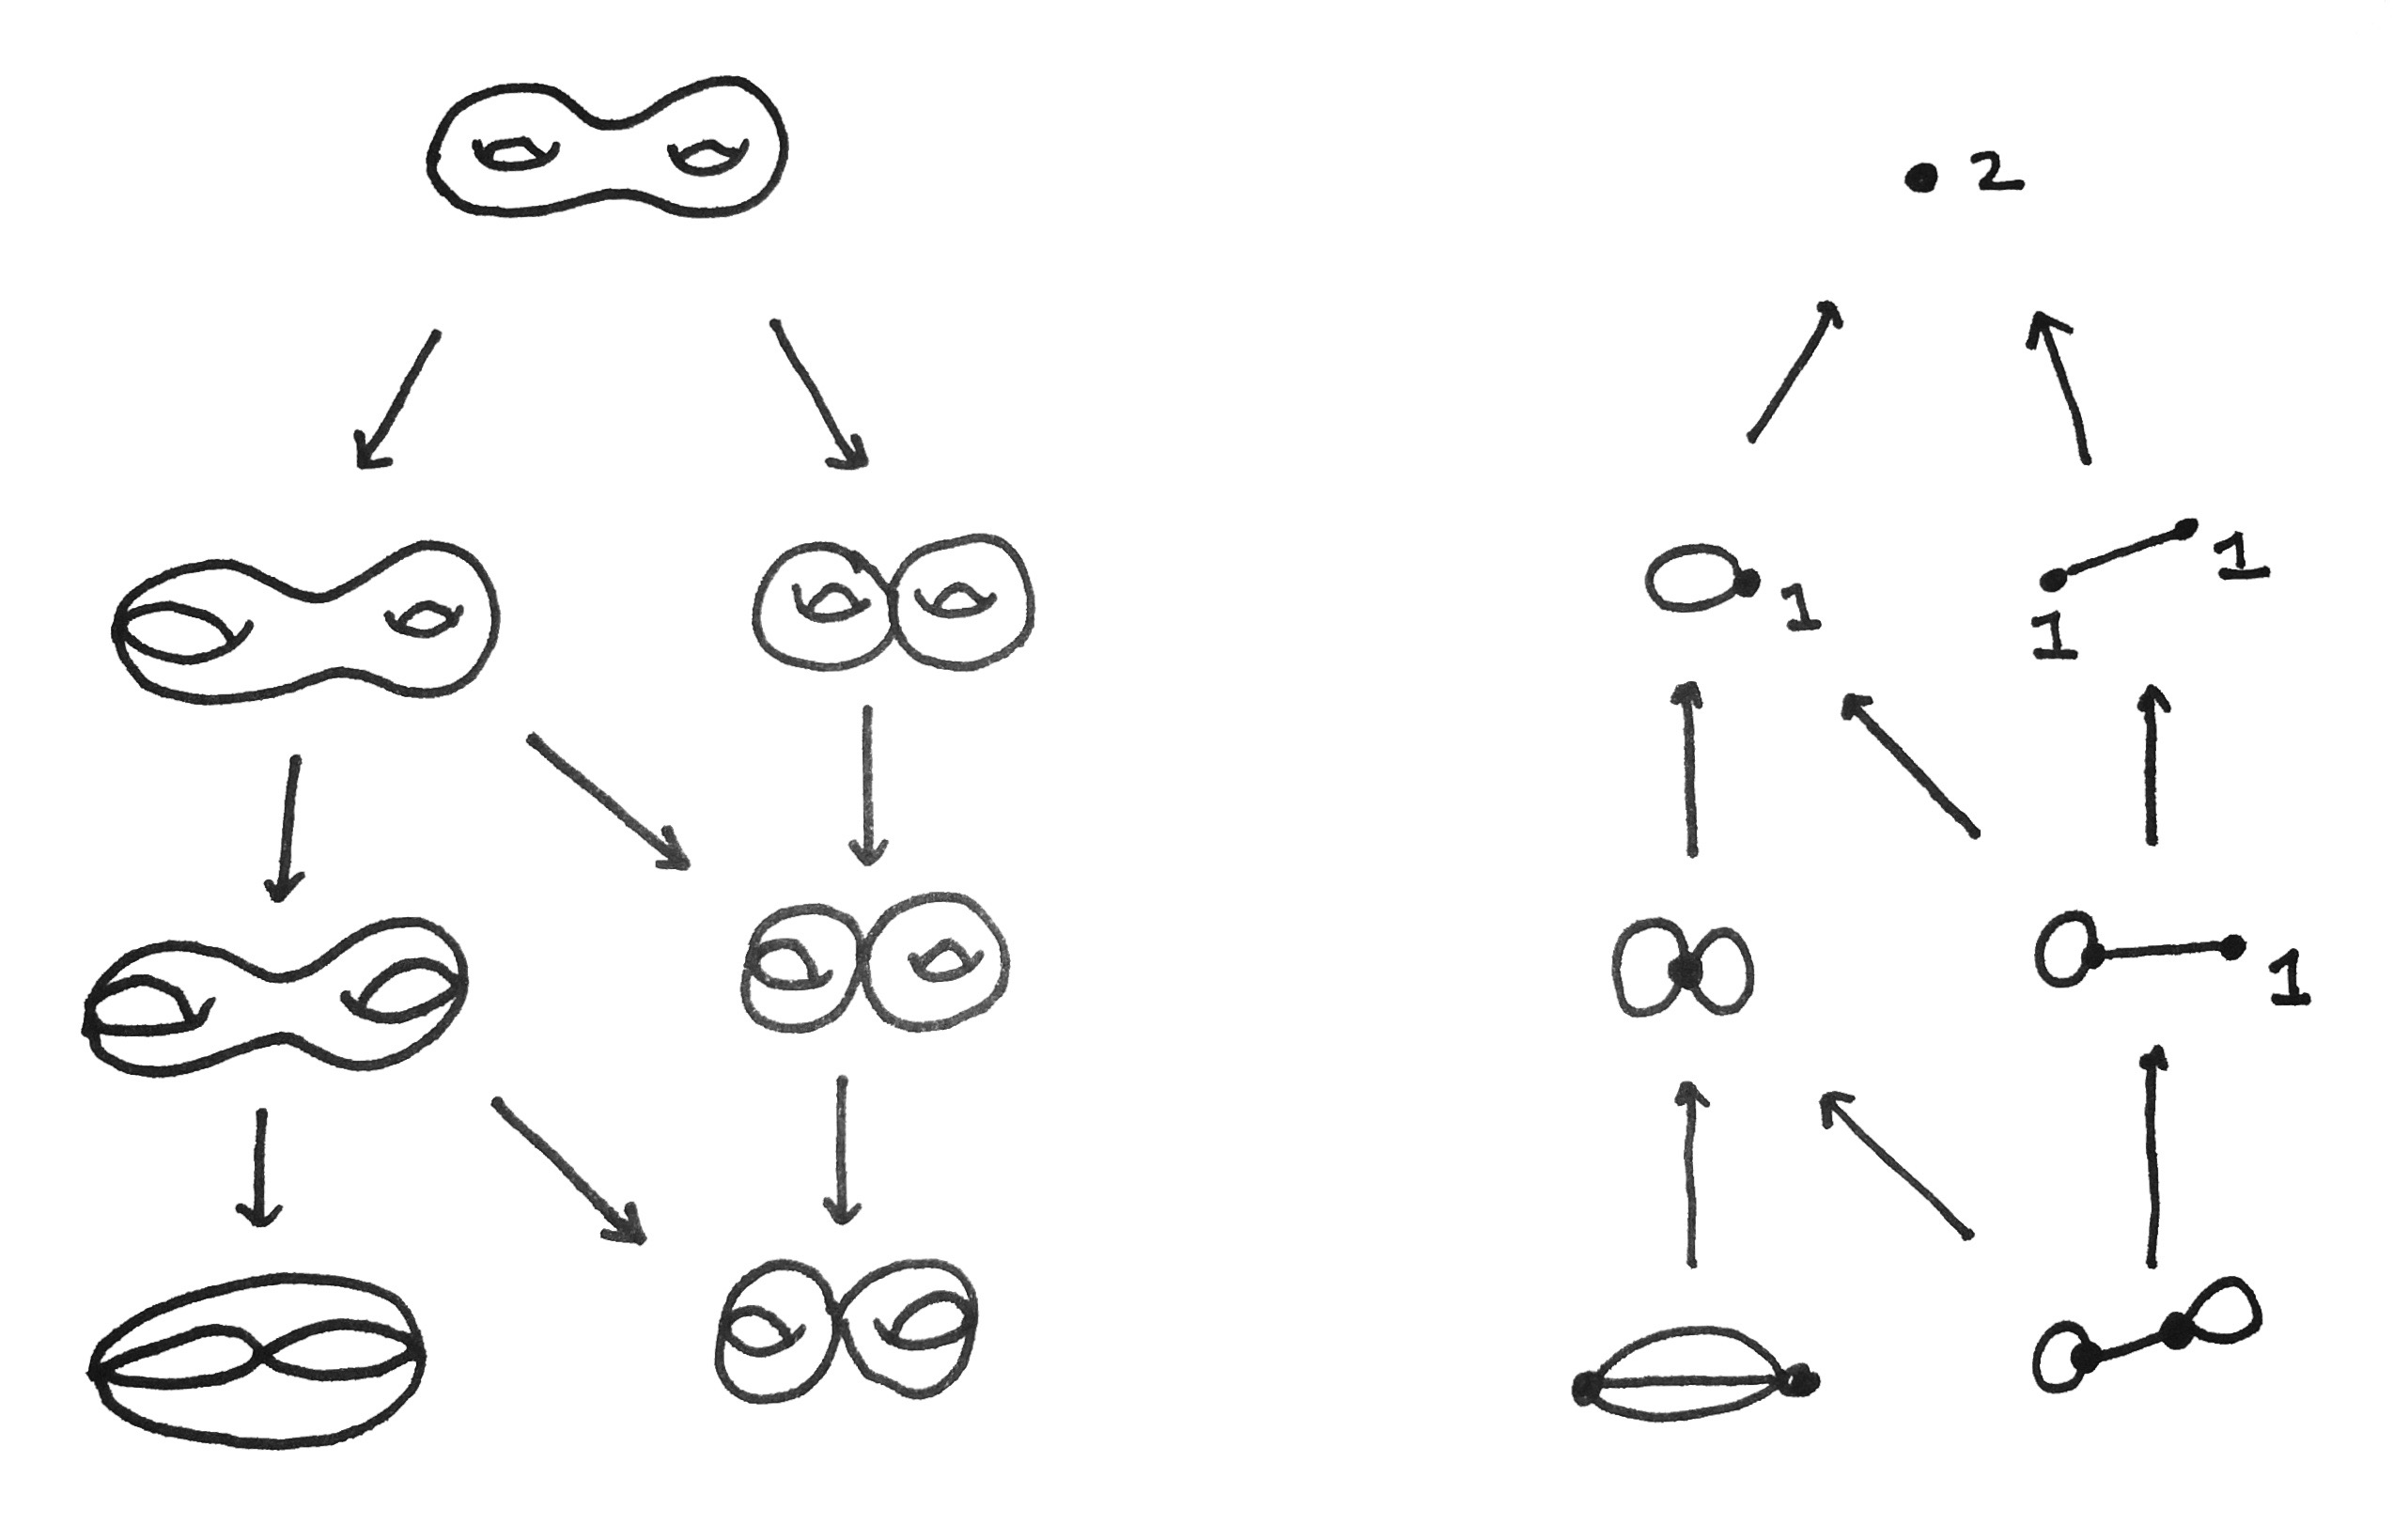
\includegraphics[width=.9\linewidth]{bijection}
\end{center}
We know that the combinatorial nature of these two moduli spaces is similar, so the natural question to ask is: what is the right way to tie these two spaces together?

\newpage
\subsubsection{The two methods}
\subsubsubsection{Method One}
Our goal is to understand the map
$$
M_2 \rightarrow M_2^{tr}.
$$
We now discuss the methods presented in \cite{section5} for carrying this out.

\begin{theorem}[\cite{section5}] There is a commutative diagram
\[
\begin{tikzcd}
M_{0,6} \arrow{r}{} \arrow[swap]{d}{} & M_{0,6}^{tr} \arrow{d}{} \\
M_2  \arrow{r}{} & M_2^{tr}
\end{tikzcd}
\]
\end{theorem}
Now, we may study the bottom map by instead studying the top horizontal map and the right vertical map, which we understand well.\\


The map from 
$$
M_{0,6} \rightarrow M_2
$$
takes the genus 2 curve coming from the hyperelliptic cover of $\mathbb{P}^1$ with the 6 marked ramification points.
All genus 2 curves are hyperelliptic, meaning any one can be defined by giving 6 points in $\mathbb{P}^1$. The curve is then the double cover of $\mathbb{P}^1$ branched at the 6 points. If the curve is given in the form
$$
y^2 = f(x).
$$
For a polynomial $f$ of degree 5 or 6, then the points are precisely the roots of $f$, plus possibly the point at infinity depending upon if $f$ is degree 5.
\\

The space $M_{0,6}^{tr}$ is one we know well: this is the space of trees with 6 taxa. Using the distances $d_{ij}$ between the 6 marked points, we get a fan in $\mathbb{TP}^{14}$. Combinatorially, it agrees with the tropical Grassmannian $trop(Gr(2,6))$, as described in \cite{tropicalbook}. We know that $M_{0,6}^{tr}$ has a tropical basis given by the Pl\"{u}cker relations for $Gr(2,6)$. It has one 0 dimensional cone, 25 rays,  105 two dimensional cones, and 105 three dimensional cones. The dimension corresponds to the number of interior edges in the tree.
Then the map
$$
M_{0,6} \rightarrow M_{0,6}^{tr}
$$
can be described as follows. Denote the 6 points in $\mathbb{P}^1$ by $(a_i: b_i)$. Then, valuations of all $2 \times 2$ minors of the matrix
$$
\begin{bmatrix}
a_1 & a_2 & \cdots & a_6 \\
b_1 & b_2 & \cdots & b_6
\end{bmatrix}.
$$
This describes a point in $\mathbb{P}^{14}$:
$$
\Delta = (p_{12}: p_{13}: \cdots: p_{56}),
$$
and this point gives a tree metric on a tree with 6 taxa by taking $d(i,j) = -2p_{ij} + \bf{1}$ for a suitable constant $n$.\\ 

The map 
$$M_{0,6}^{tr} \rightarrow M_2^{tr}$$
is a morphism of generalized cone complexes, and can be described as follows. Given a point in $M_{0,6}^{tr}$, find the tree associated to it, with interior edge lengths. This tree maps to the corresponding tropical curve, as in the figures displayed below. For example, the caterpillar tree maps to the dumbell graph. Then, we must define the lengths of the edges in the corresponding tropical curve.
 If an interior edge in the tree has length $l$ and maps to an edge in the tropical curve which contributes to the genus,
then the edge in the tropical curve receives length 2$l$. Otherwise, the edge in the tropical curve receives length $l/2$. So, in the case of the dumbell, if all interior edges of the tree have length $l$, then the two loops of the dumbell obtain length $2l$, and the edge joining them obtains length $l/2$.
 \\

There is also a map $\mathbb{P}^{14} \rightarrow \mathbb{P}^{14}$ coming from the Segre cubic which sends
\begin{align*}
(p_{12}: p_{13}: \cdots: p_{56}) \mapsto &(p_{12}p_{34}p_{56}:p_{12}p_{35}p_{46}:p_{12}p_{36}p_{45}:p_{13}p_{24}p_{56}:p_{13}p_{25}p_{46}\\
&:p_{13}p_{26}p_{45}:p_{14}p_{23}p_{56}:p_{14}p_{25}p_{36}:p_{14}p_{26}p_{35}:p_{15}p_{23}p_{46}\\
&:p_{15}p_{24}p_{36}:p_{15}p_{26}p_{34}
:p_{16}p_{23}p_{45}:p_{16}p_{24}p_{35}:p_{16}p_{25}p_{34}).
\end{align*}
Call these coordinates $m_0, \ldots, m_{14}$. Then, we can calculate the lengths in the tree using the $m_i$. For instance, in the snowflake tree, we have that the interior edge lengths will be
$$
v(m_2)-v(m_{13}),v(m_6)-v(m_{13}),v(m_{14})-v(m_{13}).
$$
 Suppose that the polynomial $f$ has roots $r_1, \ldots, r_6$. Additionally, suppose that $r_1,r_2$, and $r_3,r_4$, and $r_5,r_6$ come together in the special fiber, and let valuations of the pairwise differences be called $v_{12},v_{34}, v_{56}$. Then (after an elementary calculation) we find that the interior edge lengths in the snowflake are  $v_{12},v_{34}, v_{56}$. The example in Section \ref{example1} is a special case of this.
 
 This method for finding the tropical curve takes advantage of the fact that all genus 2 curves are hyperelliptic. This allows us to look at the space of trees on 6 taxa by mapping valuations of the differences of the roots into the tropical Grassmannian. Then, the difficult task is to find the correct scaling factors for the edge lengths in the tropical curve. For this reason, a promising direction for future work would be to study tropicalizations of hyperelliptic curves.

\begin{center}
  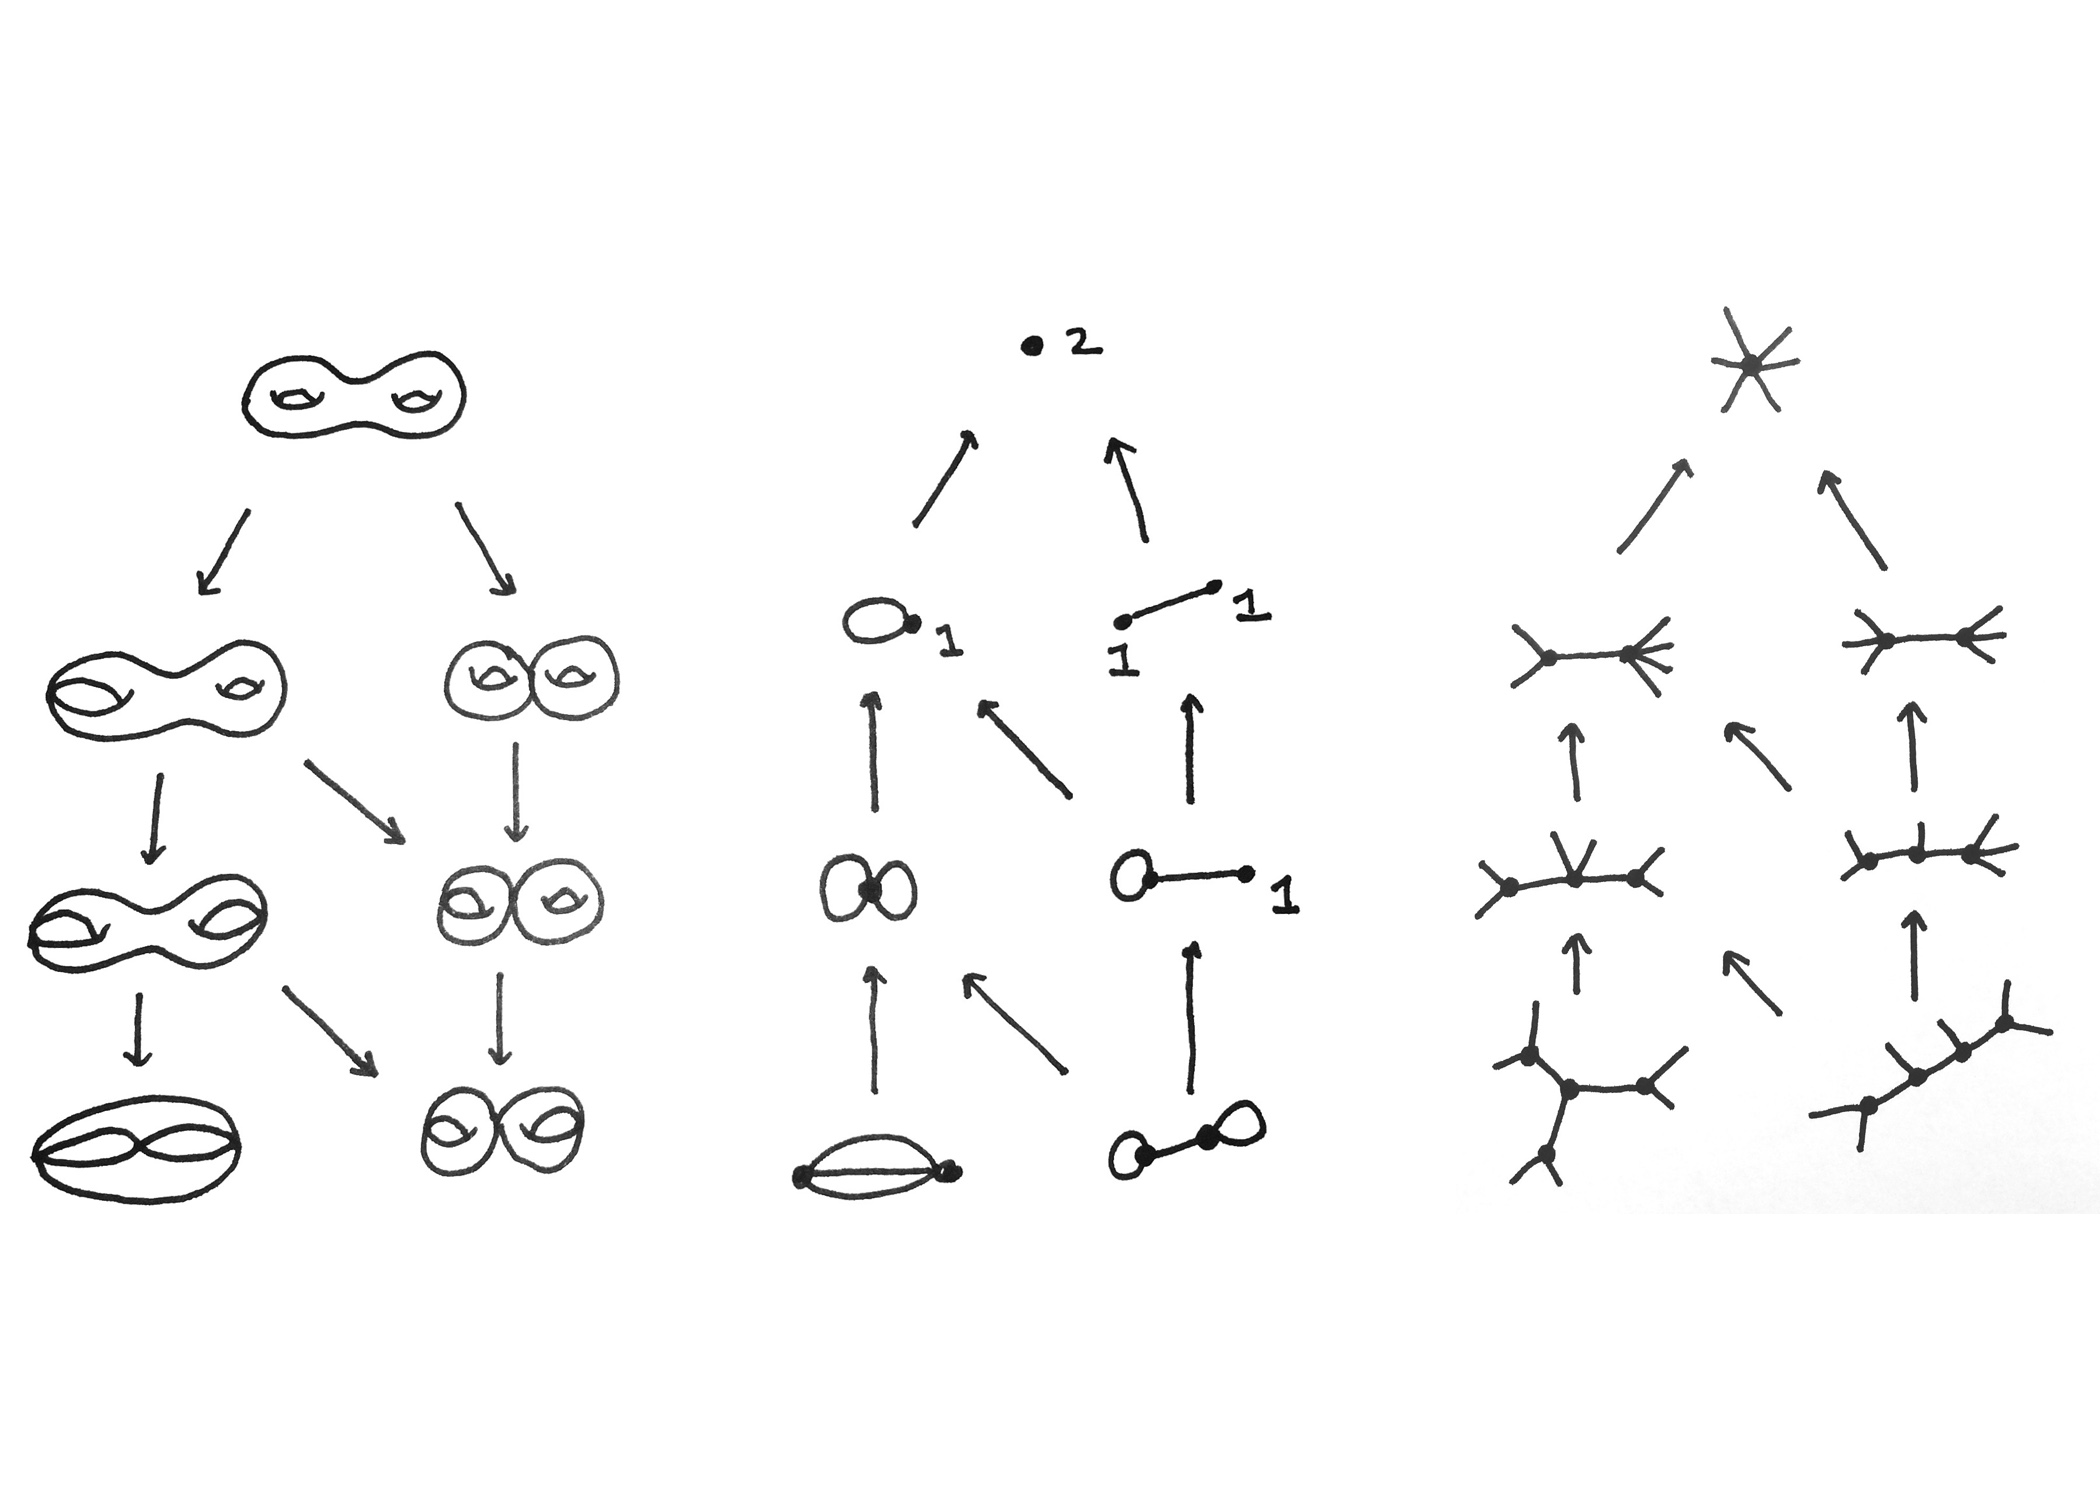
\includegraphics[width=0.9\linewidth]{curvestroptree}
\end{center}


\subsubsection{Method Two}

 In the case of genus 1 curves, the valuation of the $j$-invariant determines the semistable reduction type of the curve, so it is natural to wonder whether or not there are other invariants which play a similar role for higher genus. In \cite{masters}, Helminck completely determines the semistable reduction type of a genus two curve using the \emph{Igusa invariants}. These were first defined by Igusa in \cite{igusa}. Helminck gives the following theorem.

\begin{theorem}[\cite{masters}]
Let $C$ be a semistable curve of genus 2 over $K$. Then the cycle lengths and reduction type of a faithful tropicalization can be completely described in terms of the tropical Igusa invariants.
\end{theorem}



%As before, let $R$ be a valuation ring, let $K$ be the field of fractions, $v$ the caluation, $m$ the maximal ideal of $R$, $k$ be the residue field $R/m$. Let $C$ be a connected smooth proper curve over $K$, and $\mathcal{C}$ a model of $C$ over $R$. Let $\mathcal{C}_S$ be its special fiber. Denote the irreducible components by $\{\mathcal{C}_i\}$. Let $G$ be a finite graph whose vertices are the components $\mathcal{C}_i$ of $\mathcal{C}_S$ and let the edges correspond to intersections between the components. 

One can introduce the Igusa invariants $ \{J_2, J_4, J_6, J_8, J_{10}\}$ and $\{I_2, I_4, I_6, I_8, I_{12}\}$ of the curve $C$ as follows. Since $C$ is hyperelliptic we have that $C$ is given by an equation of the form $y^2 = f(x)$ where $f$ has degree $5$ or $6$. The exact values of the invariants can then be written down in terms of the roots of the polynomial $f$ (See the \emph{Mathematica} notebook). For instance, if the roots are $x_1, \ldots, x_6$, then
$$
J_2 = \frac{1}{8} \sum_{\text{fifteen}} (x_1-x_2)^2(x_3-x_4)^2(x_5-x_6)^2,
$$
where the sum is over all 15 ways of grouping 6 objects into pairs.

\begin{defn} The \emph{tropical Igusa invariants} are the valuations of $J_i$ and $I_i$. 
\end{defn}

Using the tropical Igusa invariants, Helminck's theorem can determine which of the seven possible reduction types $\mathcal{C}_S$. The full theorem statement may be found in \cite{masters}, and we implemented this in \emph{Mathematica} (see the appendix). Helminck also determines the \emph{thickness} of the singular points on $\mathcal{C}_S$ in terms of the tropical Igusa invariants, which gives us the lengths of the edges in the tropical curve.

\subsubsection{Examples}

\subsubsubsection{Two roots coincide}
\label{example1}

Suppose exactly two roots coincide in the residue field.
Call these two points $a_5,a_6$. Then the tropical Igusa invariants are
$$
(0, 0, 0, 0, 2a, 0, 0, 0, 0, 0),
$$
where $a = v(a_5-a_6)>0$.
This tells us that the curve is irreducible with one singular point of thickness $2a$. This corresponds to a single loop of length $2a$ and a vertex of weight 1. \\

On the other hand, in $M_{0,6}^{tr}$ we have a point of the form
$$
(0,\ldots,0,a)=(p_{1,2}, p_{1,3}, \ldots, p_{1,5}).
$$
 This gives us a tree metric
$$
(n,\ldots, n, n-2a)=(d_{1,2}, d_{1,3}, \ldots, d_{1,5}).
$$
So the tree has the desired type, with an interior edge length of $a$. Then, we double this length to find the length of the corresponding loop in the tropical curve.
 \begin{figure}[h]
\centering
  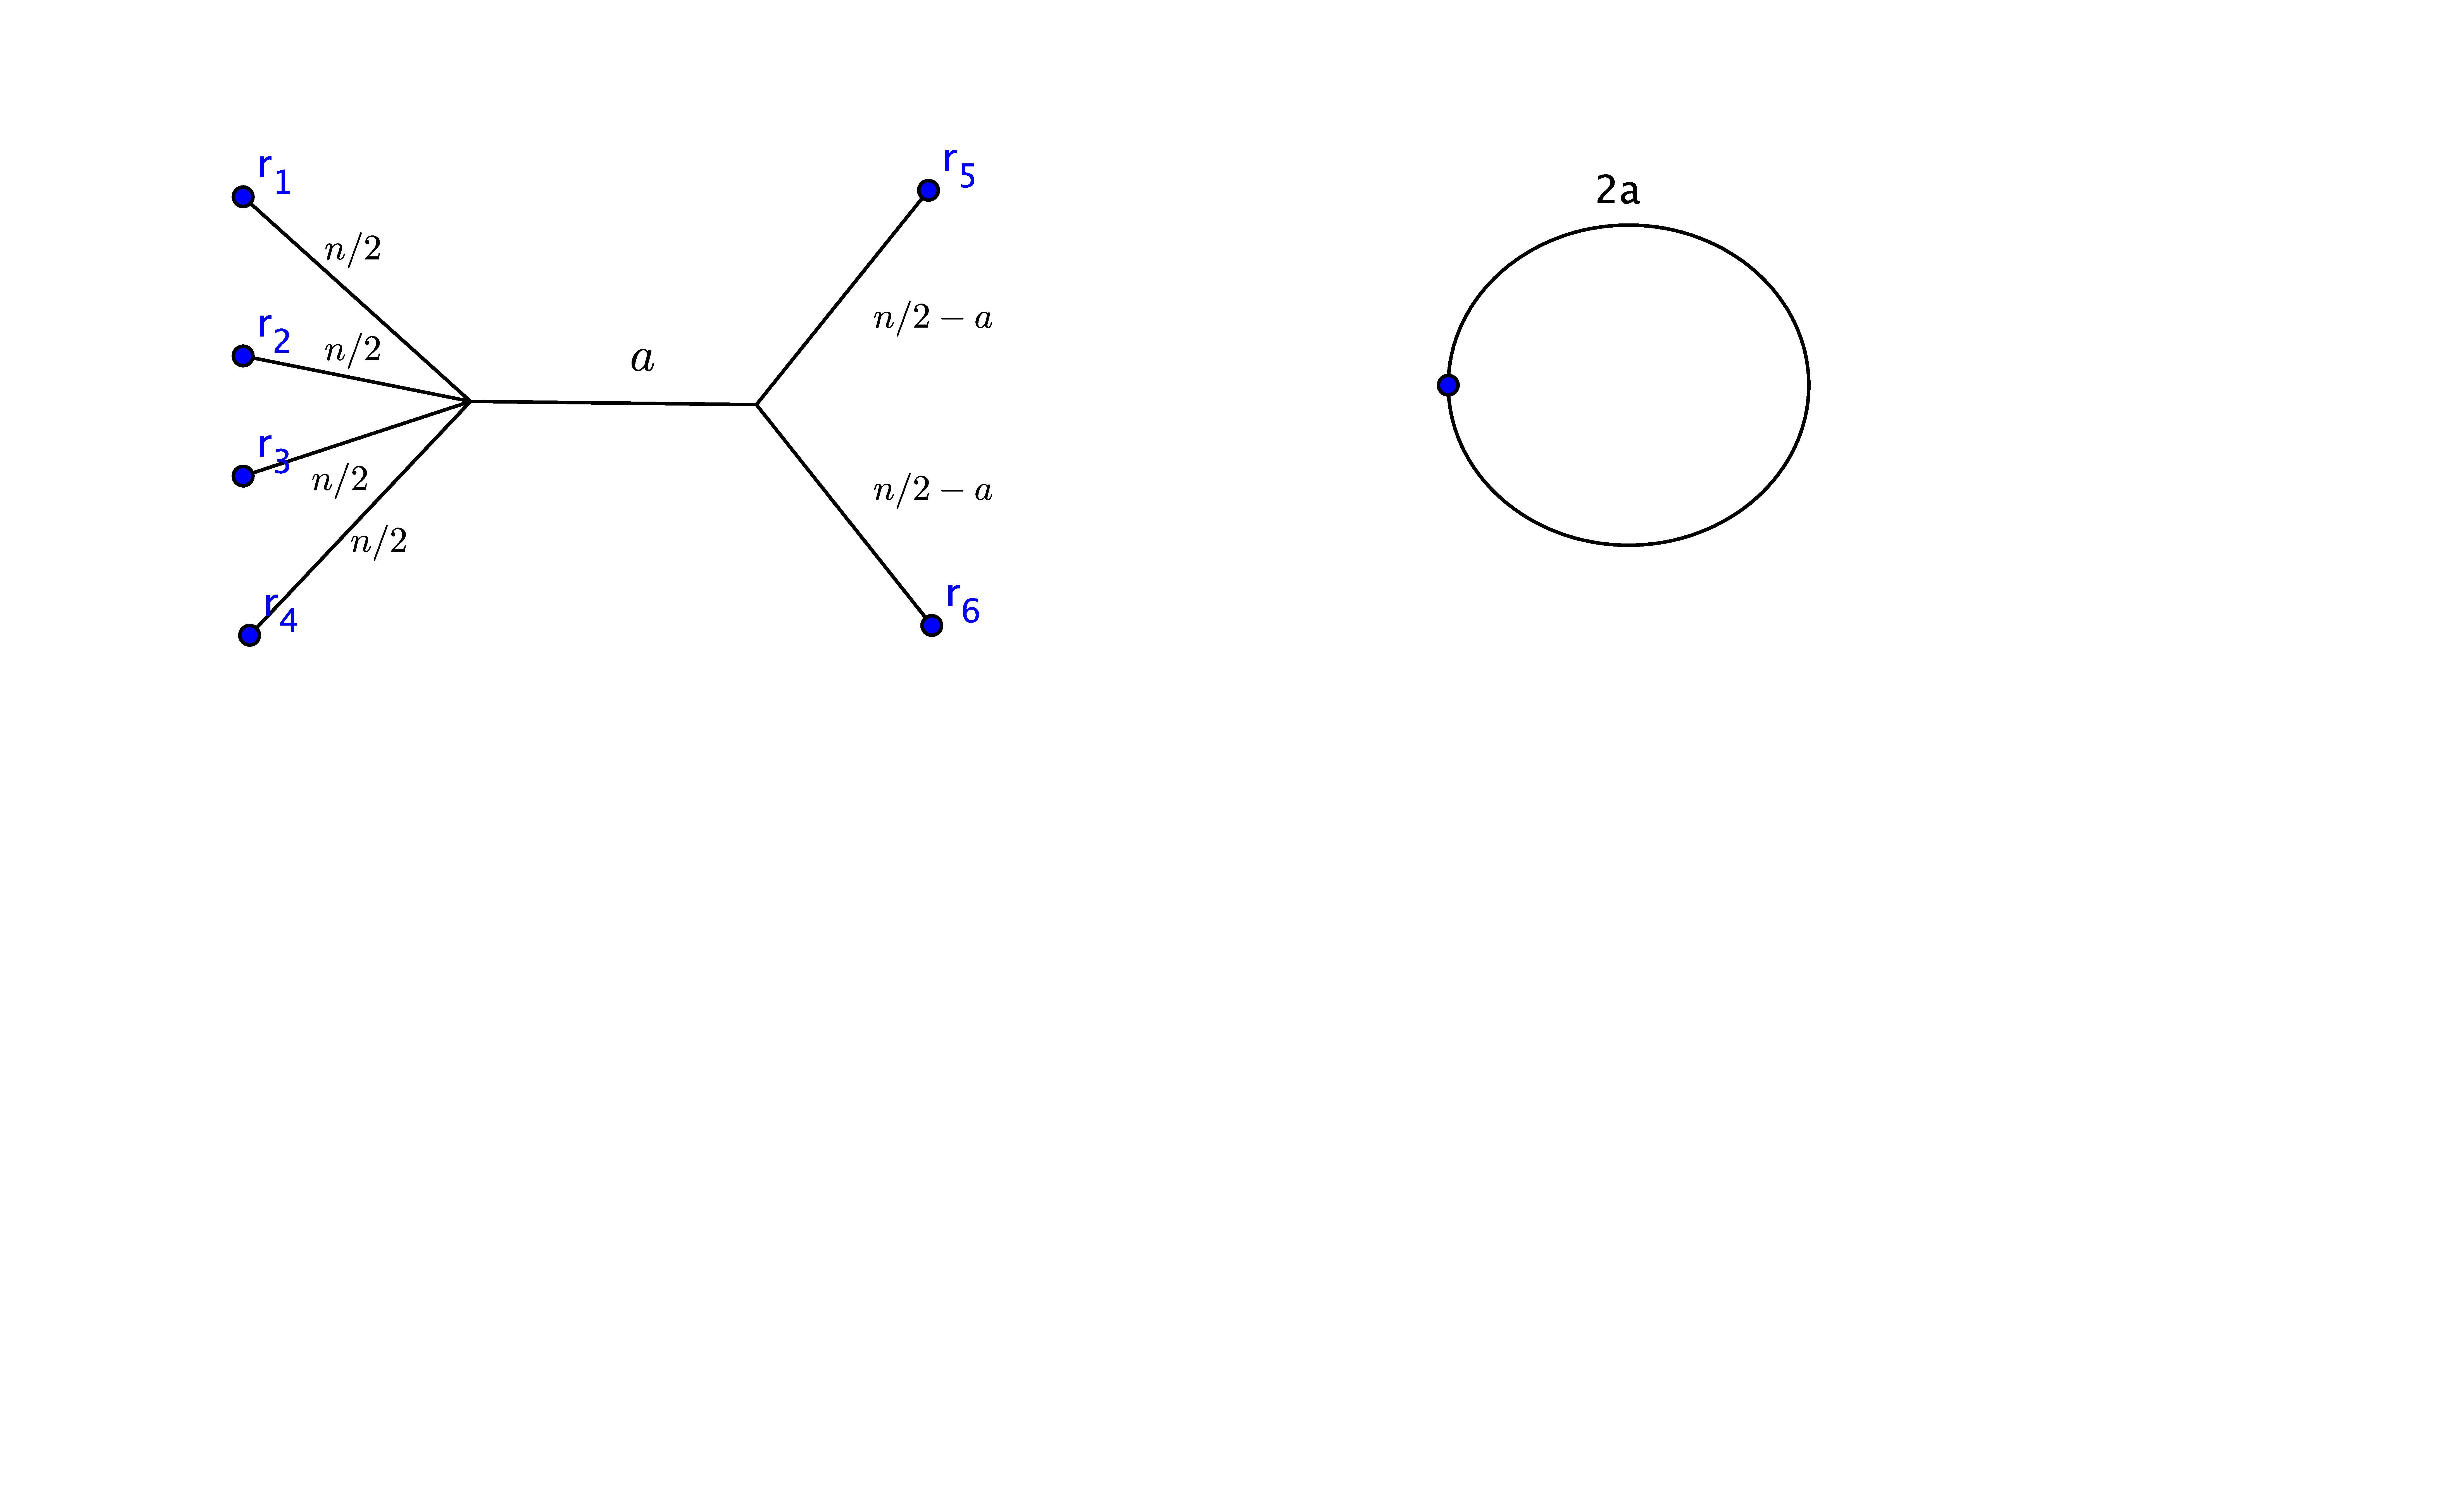
\includegraphics[width=.7\linewidth]{ex1.pdf}
\end{figure}

We see that in both cases, we obtained the same result using the two methods.
 
 
 
\subsubsubsection{A Snowflake}

Consider the polynomial
$$
y^2 = (x-1)(x-2)(x-3)(x-6)(x-7)(x-8),
$$
with the 5-adic valuation.
Its tropical Igusa invariants are
$$(0, 2, 2, 2, 6, 0, 0, 2, 2, 2).$$
 This tells us that the reduction type is two projective lines intersecting in three points, with thicknesses $(2,2,2)$, so the graph is the theta graph with each edge having length 2.\\

On the other hand, in $M_{0,6}^{tr}$ we have the point
$$
(0, 0, 1, 0, 0, 0, 0, 1, 0, 0, 0, 1, 0, 0, 0) = (p_{1,2}, p_{1,3}, \ldots, p_{1,5}).
$$
So that a possible tree metric (up to all 1's vector) is
$$
(4, 4, 2, 4, 4, 4, 4, 2, 4, 4, 4, 2, 4, 4, 4) =  (d_{1,2}, d_{1,3}, \ldots, d_{1,5}).
$$
This means that this is a metric for the snowflake with edge length 1 on each interior edge, so this corresponds to a theta graph with edges of length 2.


 \begin{figure}[h]
\centering
  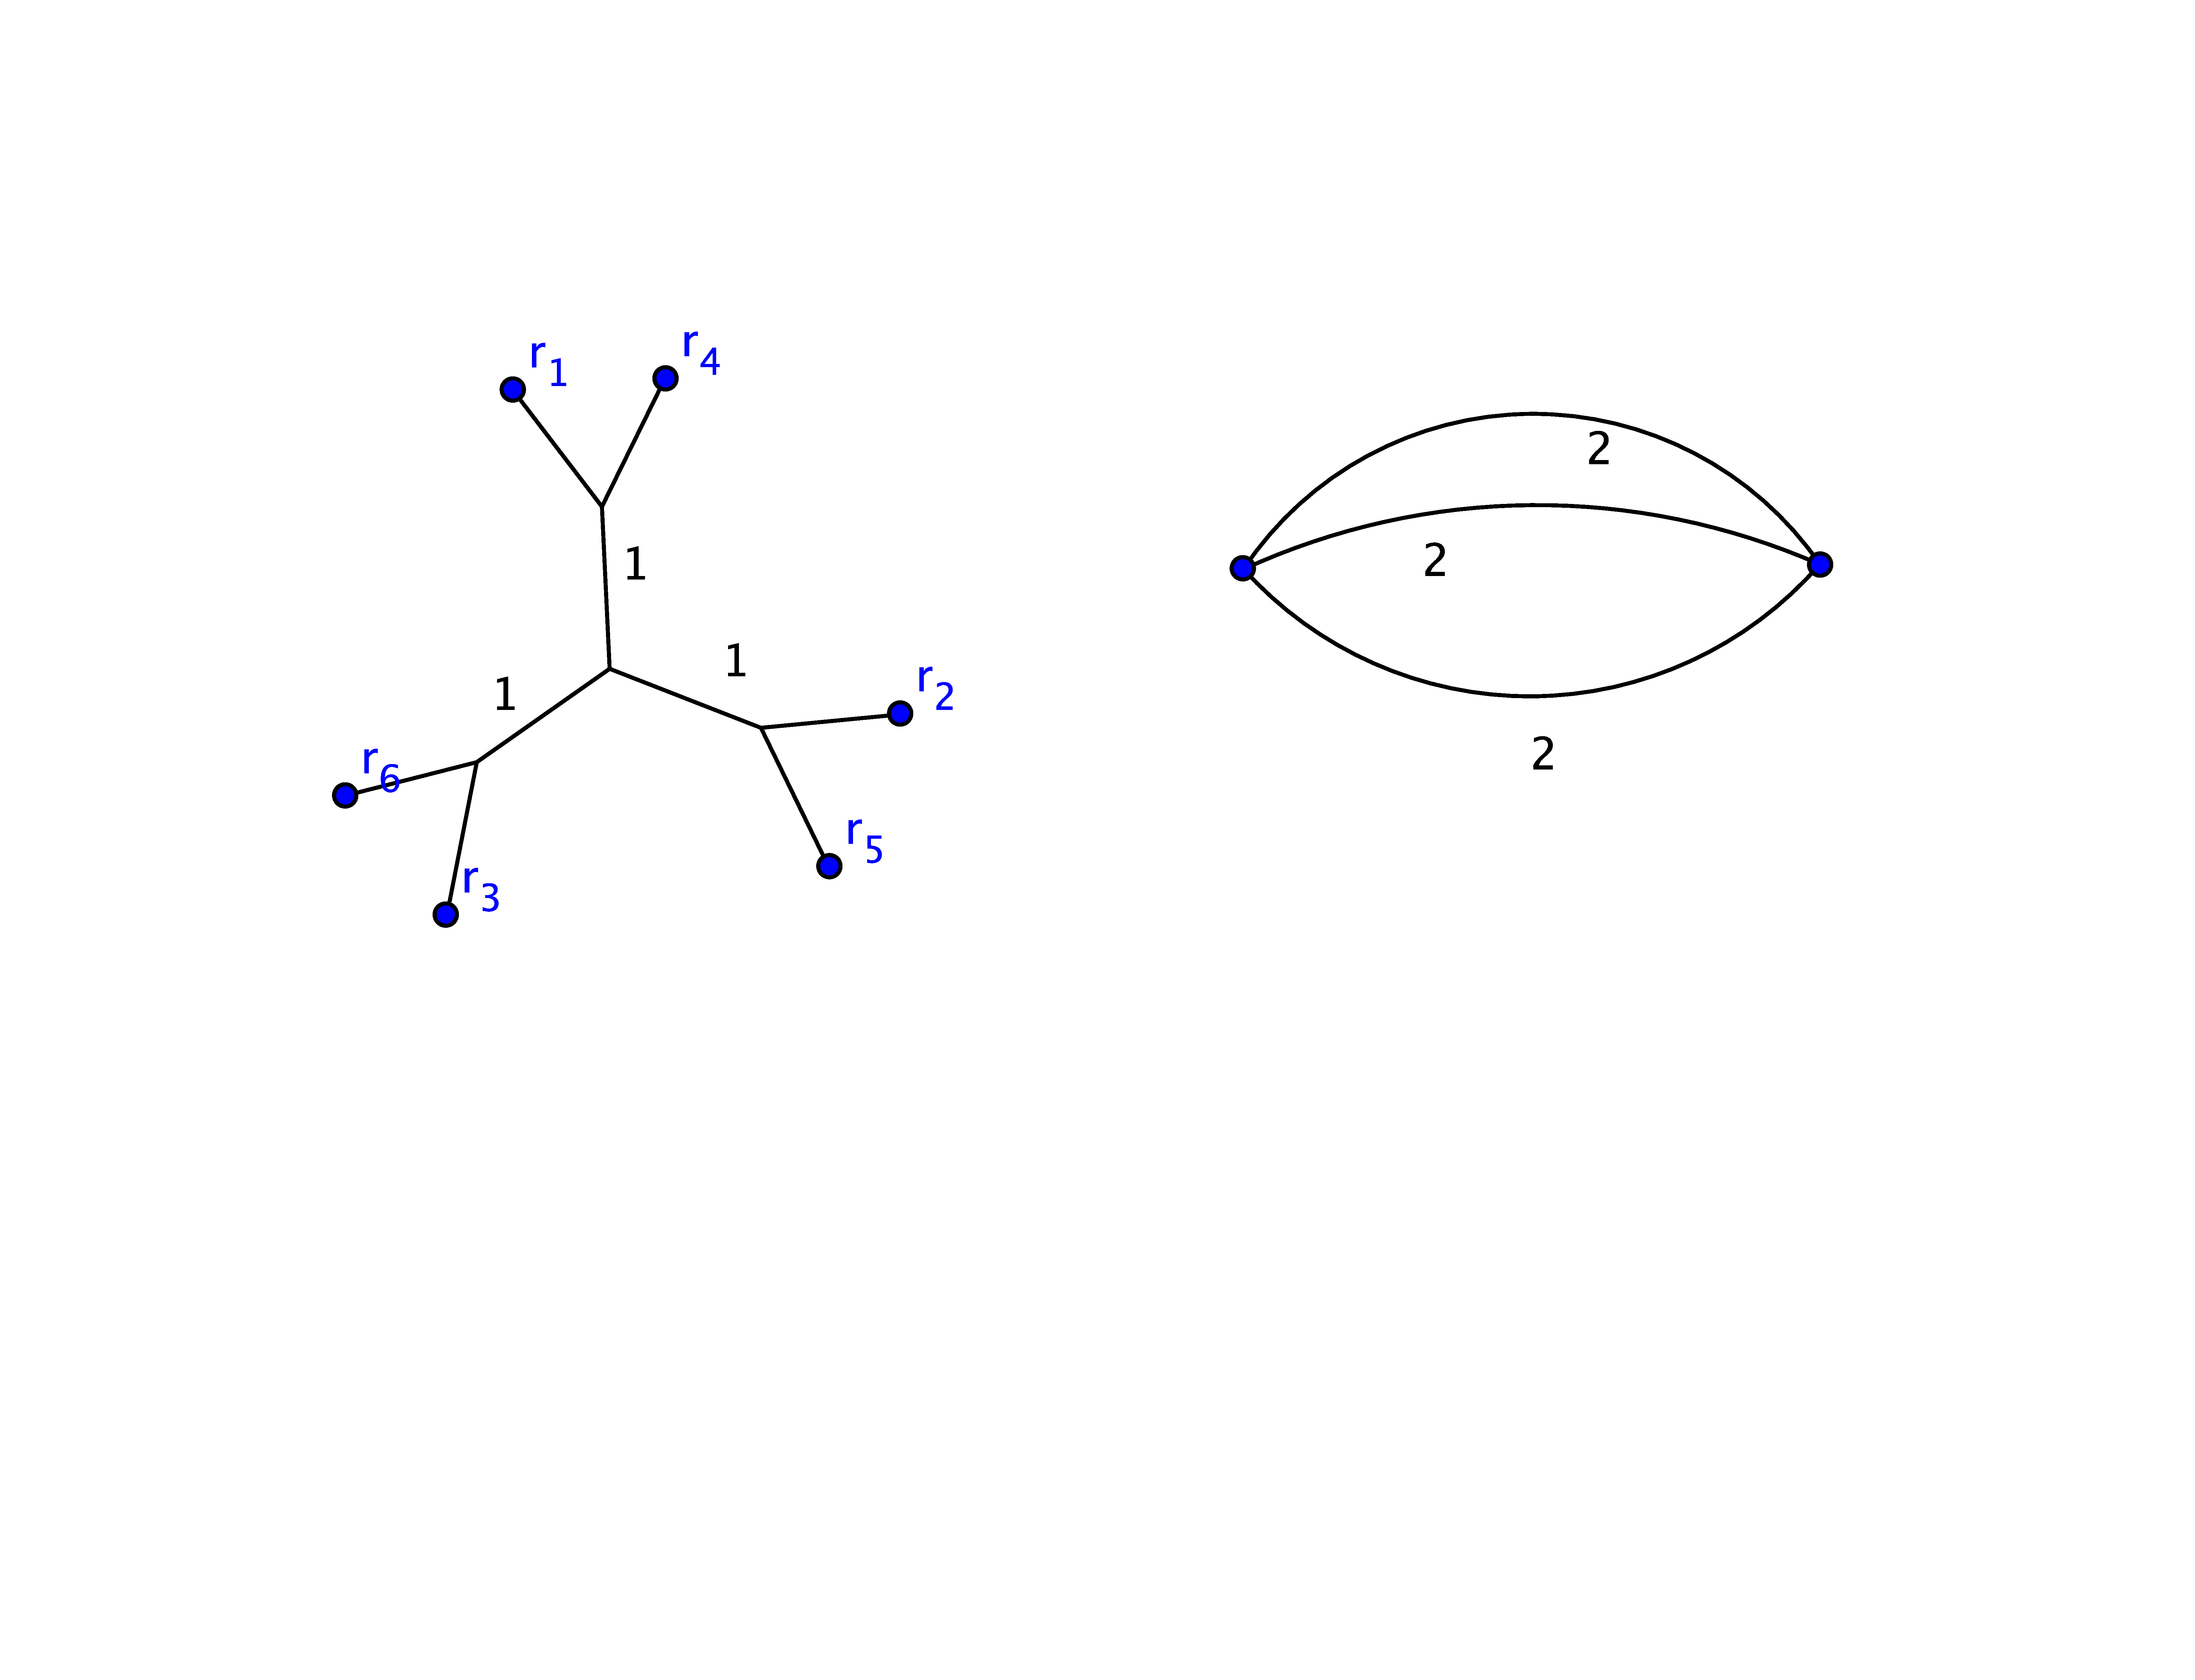
\includegraphics[width=.75\linewidth]{ex2.pdf}
\end{figure}

